\section{Introduction}

Increasingly, objects in our built environment are equipped with computation and communication, making them potential targets for user interaction. Such interactions might be {\em explicit} -- controlling smart appliances such as intelligent lighting, AV equipment, or HVAC systems; or {\em implicit} -- tracking the user's attention to gauge interest e.g., for advertising or context-aware computing \bjoern{second part needs to be stronger}. Both uses rely on {\em selection} information by which a system keeps track of the user's {\em locus of attention}~\cite{raskin} in the world.

Past research has introduced techniques of augmenting hand-held mobile devices with accessories like laser pointers to enable direct aiming at target devices in space~\cite{beigl_point_1999,patel_2-way_2003}. While promising, some drawbacks of using handheld devices are that the device first has to be retrieved (e.g., from a pocket) and consciously aimed (which also limits use to explicit scenarios); that the user's hands are required to be free for operation (one to hold the device, one to operate the touch screen); and that the user's visual attention is now split between looking down at a screen and out at targets in the world. 

Emerging head-worn computing devices have the potential to overcome some of these limitations: because they are worn, they do not require retrieval; they may enable hands-free or uni-manual interactions; and they offer near-eye or see-through displays to overlay information. \bjoern{needs a bridge from head-worn device to using head orientation as a feature}.

In this paper, we investigate how to leverage head-orientation for target selection in physical spaces. We characterize this interaction modality because it can readily be implemented with small hardware changes to emerging wearable devices. We augment Google Glass\footnote{\url{http://www.google.com/glass/start/}} with custom hardware for this purpose. We use infrared (IR) communication between Glass and target appliances to establish a connection; and on wireless 802.15.4 radio communication to exchange control messages.  
%Glass is augmented with a narrow-beam IR emitter and a 802.15.4 radio. Target appliances similarly have IR receivers and radios.

Users look in the direction of a target they wish to acquire to initiate interaction (e.g., at a lamp to control lighting, or at a speaker to change music playback volume), then tap to confirm selection.  
%
Head orientation is a useful but imprecise indicator of the user's locus of attention: it contains the general direction, but not the particular point of focus. Therefore, it requires area selection \bjoern{reference} combined with disambiguation techniques.
In practice, our IR beam's selection area has a diameter of 60-120cm at distances up to 5m.
If multiple targets fall within communication range, targets compare received IR light intensity readings to disambiguate. Users can override this default selection with an  on-screen target list.

%This combination enables users to initiate interaction by orienting their head; but once initiated, users are free to look away from the target appliances while issuing control commands.

While prior work has tended to focus on proofs-of-concept, we also contribute empirical data on the system performance, usability, and user experience of head-orientation targeting and device control. We first report measurements of range and beam characteristics of our controller. We then conduct a study with $14$ participants that compares acquisition times for physical targets in a room for our technique and an alternative list selection interface. We find that target acquisition through head orientation is preferred by users and is faster than list selection, given the constraints of linear input using a head-worn touch controller. 
We then quantify the additional benefit of using IR-intensity disambiguation \bjoern{and find XYZ.}
%
\bjoern{Say something about the inferred map if we get around to it}.

We then demonstrate how the technique can be applied to a "universal remote control" scenario. In our implementation, user look at a target appliance and tap to load an appliance-specific control UI on the head-mounted display, which enables adjustment of discrete and continuous parameters through a touchpad interface (Figure~\ref{fig:teaser}) \bjoern{we may need a different figure 1 with the changed focus of the paper}. We also report qualitative results from users performing  home automation tasks with this system.

\begin{figure}[t]
\centering
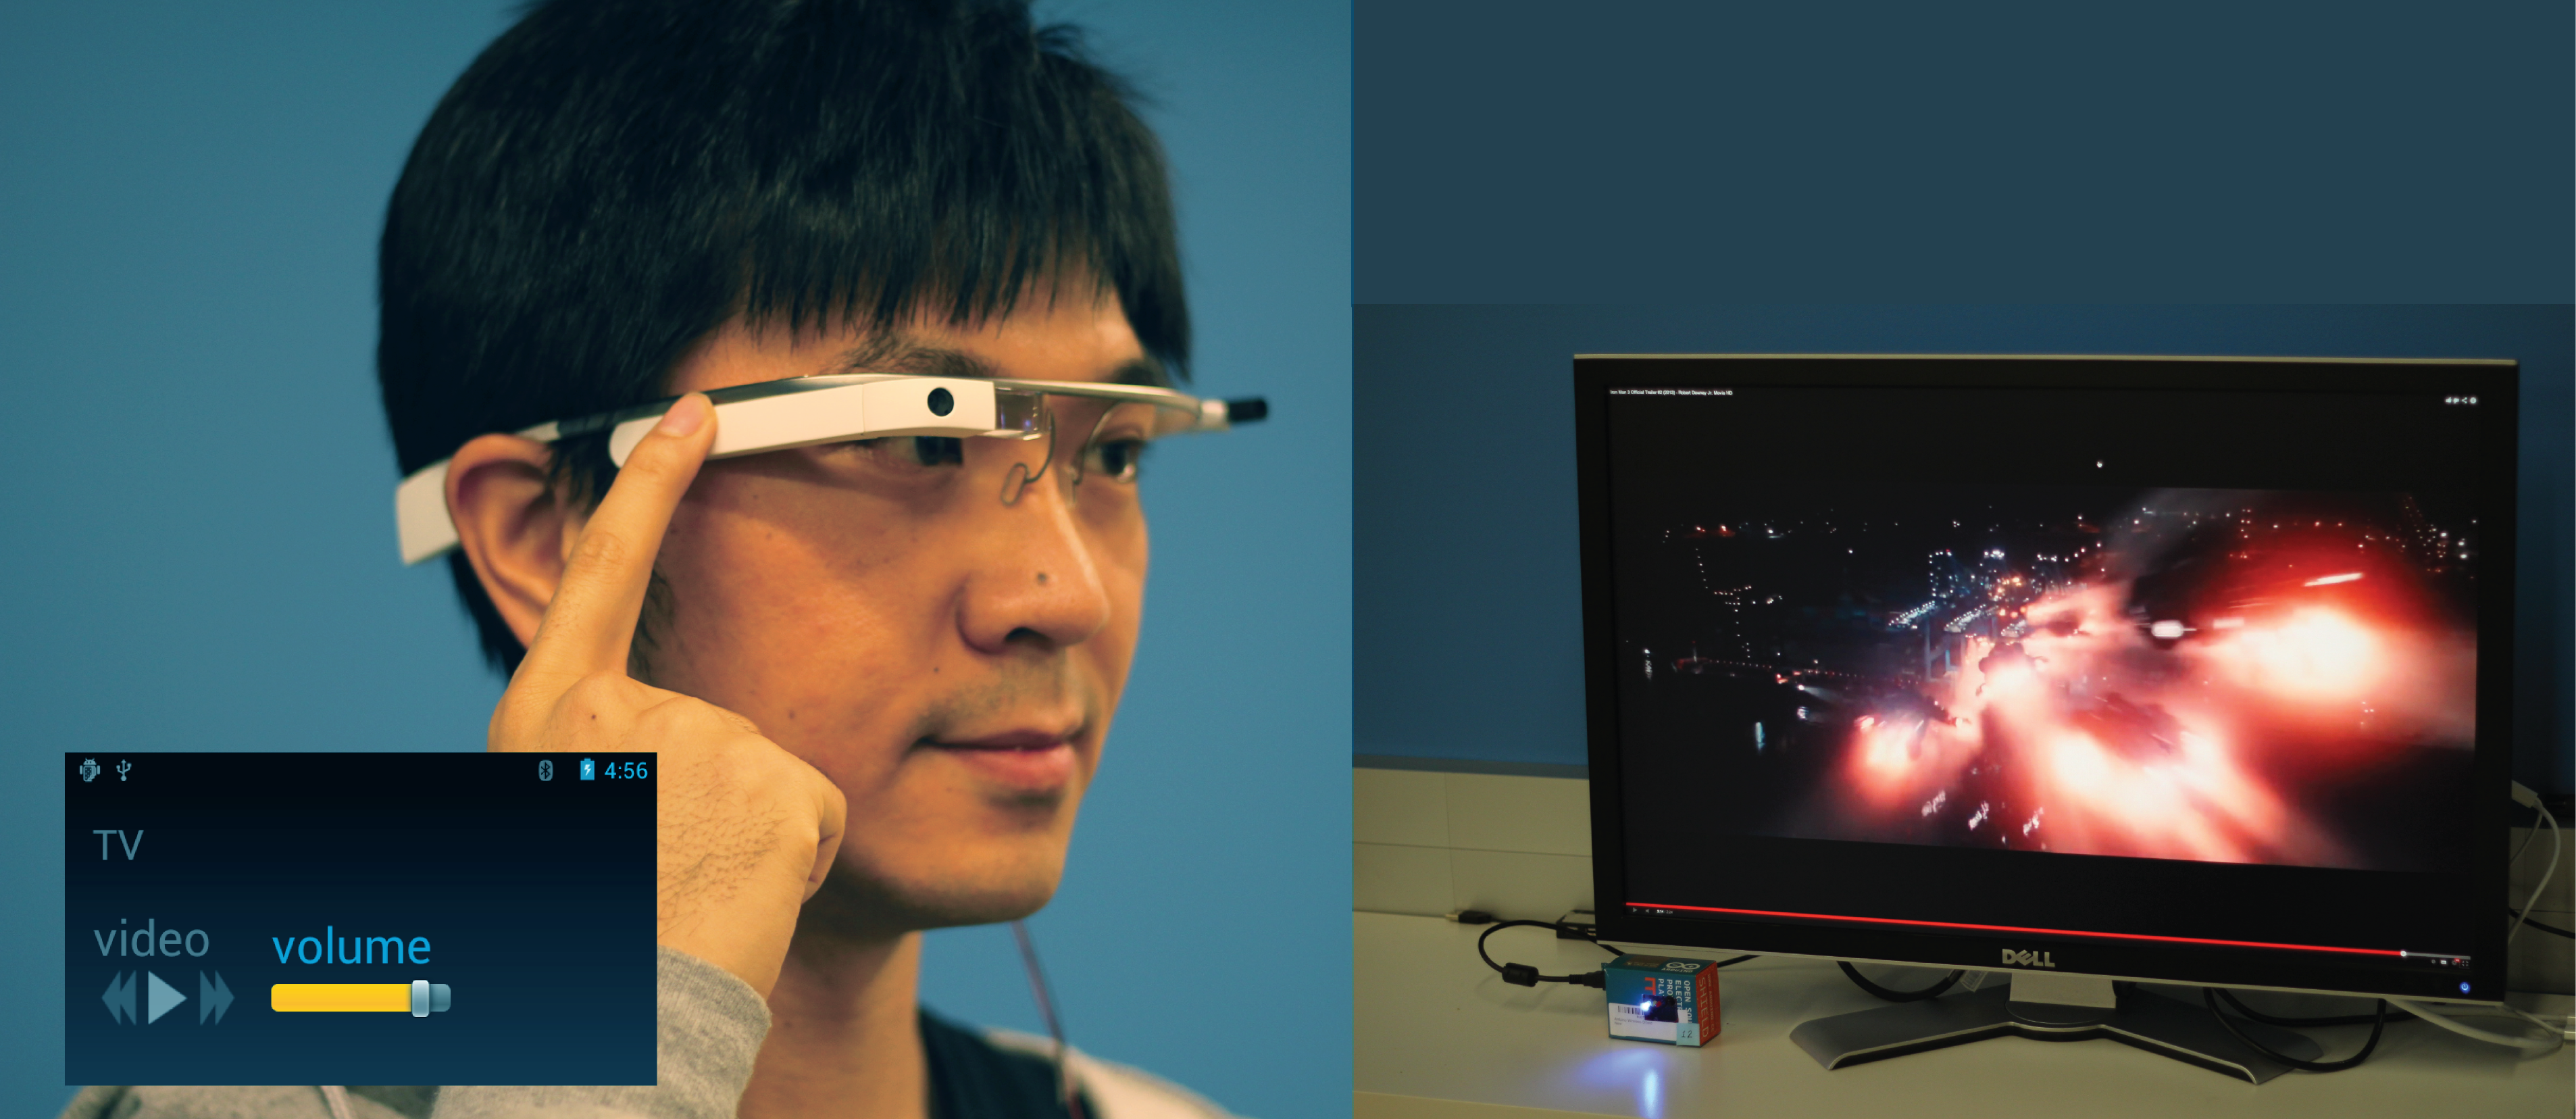
\includegraphics[width=1.0\columnwidth]{figures/teaser.jpg}
\caption{Using an augmented head-worn device (1), users can control smart home appliances (2) with head orientation targeting. A near-eye display then shows an appliance control UI (3), which users navigate through multitouch gestures.}
\label{fig:teaser}
\end{figure}








